\documentclass[tikz,border=4pt]{standalone}
\usetikzlibrary{arrows.meta,positioning}
\begin{document}
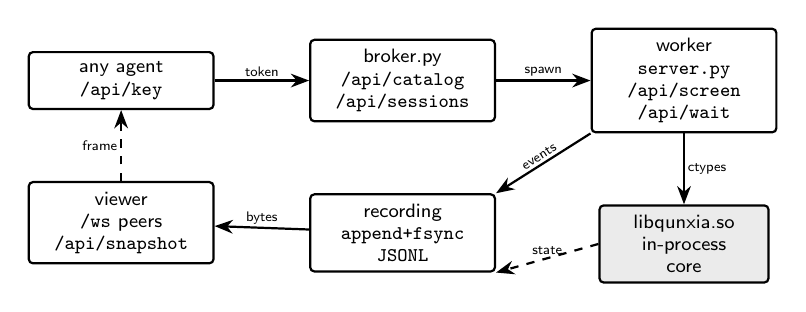
\begin{tikzpicture}[
  >=Stealth, node distance=9mm and 12mm,
  box/.style={draw, thick, rounded corners=1.5pt, align=center,
              inner sep=3.5pt, font=\sffamily\scriptsize, text width=21mm,
              minimum height=7mm},
  core/.style={box, fill=black!8, text width=19mm},
  ar/.style={thick, ->},
  lb/.style={font=\sffamily\tiny, inner sep=1pt},
]
\node[box] (agent)  {any agent\\ \texttt{/api/key}};
\node[box, right=of agent] (broker) {broker.py\\ \texttt{/api/catalog}\\ \texttt{/api/sessions}};
\node[box, right=of broker] (work)  {worker\\ \texttt{server.py}\\ \texttt{/api/screen}\\ \texttt{/api/wait}};
\node[core, below=of work] (qun)    {libqunxia.so\\ in-process\\ core};
\node[box, below=of broker] (rec)   {recording\\ \texttt{append+fsync}\\ \texttt{JSONL}};
\node[box, below=of agent] (vis)    {viewer\\ \texttt{/ws} peers\\ \texttt{/api/snapshot}};

\draw[ar] (agent) -- node[lb, above]{token} (broker);
\draw[ar] (broker) -- node[lb, above]{spawn} (work);
\draw[ar] (work) -- node[lb, right]{ctypes} (qun);
\draw[ar] (work.south west) -- node[lb, above, sloped]{events} (rec.north east);
\draw[ar] (rec) -- node[lb, above]{bytes} (vis);
\draw[ar, dashed] (qun.west) -- node[lb, above]{state} (rec.south east);
\draw[ar, dashed] (vis.north) -- node[lb, left]{frame} (agent.south);
\end{tikzpicture}
\end{document}
